\documentclass[sigconf,review,anonymous]{acmart}
\acmConference[ESEC/FSE 2018]{The 26th ACM Joint European Software Engineering Conference and Symposium on the Foundations of Software Engineering}{4–9 November, 2018}{Lake Buena Vista, Florida, United States}
\usepackage{pdftexcmds}
%\usepackage[pdftex]{graphicx}
\usepackage{multirow}
\usepackage{pgfplots}
\usepackage{tikz}
\usepackage{balance}
\usepackage{amssymb, marvosym}
\usepackage{threeparttable}
%\usepackage[bookmarks=false]{hyperref}
\usepackage{url}
\PassOptionsToPackage{hyphens}{url}
\hypersetup{colorlinks=true,breaklinks=true}
\usetikzlibrary{patterns,shapes,arrows}
\newcommand\tab[1][.5cm]{\hspace*{#1}}
\hyphenation{op-tical net-works semi-conduc-tor}
\raggedbottom
\newcommand{\tool}{\textsl{tool-recommender-bot}}

\begin{document}

% Copyright
\setcopyright{acmlicensed}

\title{\tool}

\author{Chris Brown and Emerson Murphy-Hill}
\affiliation{%
	\institution{North Carolina State University}
	\city{Raleigh}
	\state{NC}
}
\email{dcbrow10@ncsu.edu, emerson@csc.ncsu.edu}

\begin{abstract}
To increase software engineer productivity, toolsmiths create tools and features to automatically complete software development tasks. However, these useful tools are often undiscovered or ignored by developers, which is problematic for software applications that rely on programmer efficiency and correctness. This paper introduces a new approach to making software engineering tool recommendations that integrates characteristics from user-to-user suggestions and industry practices for researchers to increase awareness of their products among developers. To help improve tool adoption among software engineers, we implemented this approach in \tool, an automated recommendation system, and found our design is more effective for increasing tool discovery compared to other styles of tool recommendations.
\end{abstract}
\keywords{Tool Recommendations; Tool Discovery;}

\maketitle

\section{Introduction}

To maintain and meet rising demands for technology, software engineers emphasize \textit{software quality} throughout the development process, monitoring metrics that impact software producers and consumers~\cite{KitchenhamQualityTarget}. However, despite increased attention to quality, buggy code remains a problem as the number of software errors increases~\cite{HaveThingsChanged}. The Software Fail Watch by Tricentis suggests software failures impacted 3.7 billion users and caused \$1.7 trillion in financial losses in 2017.\footnote{https://www.tricentis.com/software-fail-watch/} Additionally, the process of finding and fixing bugs, or debugging, is a time-consuming and costly activity. The National Institute of Standards and Technology reported software engineers spend 70-80\% of work time debugging and on average one error takes 17.4 hours to debug~\cite{NIST}. Finding and fixing defects early during development is also important since studies show debugging costs increase the longer a bug remains in code~\cite{SEEconomics, SoftwareAssuranceSDLC}.

To improve code quality, researchers and toolsmiths have created software engineering tools to aid developers in their work. Research shows that tools for static analysis~\cite{UsingStaticAnalysis}, refactoring~\cite{Murphy-HillFitness}, security, and more are beneficial for improving code and preventing bugs. These tools can automatically perform a wide variety of software development tasks to save time and effort for developers. Additionally, the Software Engineering Body of Knowledge recommends using development tools because they can be used to achieve ``desirable characteristics of software products''~\cite{SWEBOK}. Software enginering tools are useful for reducing software errors and debugging costs while increasing developer productivity.

Although software quality is important, development tools created to improve code are often ignored~\cite{Ivanov2017Gaps}. Previous work explores barriers preventing software engineers from adopting new tools: Tilley and colleagues studied challenges of adopting research-off-the-shelf tools in industry~\cite{Tilley2003ROTS}; Johnson and colleagues reported reasons why software engineers don't use static analysis tools~\cite{Johnson2013Why}; and Xiao and colleagues examined barriers of using security tools to prevent vulnerabilities and malicious attacks~\cite{Xiao2014Security}. One of the main barriers to tool adoption is the discoverability barrier, where users are unaware tools exist~\cite{Murphy-HillScreencastingDiscovery}. Lack of software engineering tool usage can lead to poor code quality, inconvenienced users, and significant amounts of time and money spent fixing errors. Many existing automated approaches have been implemented to increase awareness of software tools and features, but Murphy-Hill and colleagues found that developers prefer learning about tools from colleagues during normal work activities, or \textit{peer interaction}~\cite{MurphyHill2011PeerInteraction}.

To help solve the tool discovery problem among software engineers, we developed an approach for making automated tool recommendations. Our approach integrates characteristics of peer interactions and software engineering practices, and can accomodate many different types of software engineering tools to make customized suggestions to developers. Our technique is based on three main design pillars- \textit{commend}, \textit{apprehend}, and \textit{recommend}. These principles differentiate our approach from existing recommender methods and help improve the effectiveness of automated tool recommendations.

%\noindent
%TODO: Research questions?
%\textbf{RQ1:} How applicable is \tool~to real-world software applications?  \\ 
%\textbf{RQ2:} How useful are recommendations from \tool~to developers?  \\

To evaluate our approach, we implemented \tool. Our initial implementation of \tool~for this study recommends \textsc{Error Prone}\footnote{http://errorprone.info}, an open source static analysis tool for Java code, to developers on GitHub\footnote{https://github.com}, a popular code hosting and collaboration website. We measured the effectiveness of our system by observing the frequency of recommendations and how developers reacted to receiving suggestions from our system. This research makes the following contributions:

\begin{itemize}
 \item a novel approach for recommender systems to increase awareness of software engineering tools, and
 \item an implementation and evaluation of \tool~recommending a static analysis tool to developers.
 \end{itemize}

\section{Related Work}
%TODO: Use related work from whatever conference committee
This work builds on previous research examining recommendation systems in software engineering, techniques for learning new tools, approaches for tool recommendations, and existing automated recommendation systems that recommend software engineering tools.

There are numerous existing technical approaches created to solve the tool discovery problem. Fischer and colleagues found that systems requiring users to explicitly seek help, or passive help systems, are ineffective and active help systems are more useful for increasing tool awareness~\cite{Fischer1984ActiveHelpSystems}. Gordon and colleagues developed Codepourri, a system using crowdsourcing to make recommendations for Python code~\cite{Gordon2015Codepourri}. Linton and colleagues designed a recommender system called OWL (organization-wide learning) to disseminate tool knowledge using logs throughout a company~\cite{Linton2000OWL}. ToolBox was developed as a ``community sensitive help system'' by Maltzahn to recommend Unix commands~\cite{Maltzahn1995Toolbox}. Answer Garden helps users discover new tools based on common questions asked by colleagues~\cite{Ackerman1990AnswerGarden}. SpyGlass automatically recommends tools to help users navigate code~\cite{Viriyakattiyaporn2010Spyglass}. We developed \tool~to actively suggest useful programming tools and increase awareness for software engineers. Our approach differs from existing recommendation systems in the design and implementation of our tool.

\section{Approach}

Our approach uses three design pillars to increase awareness of software engineering tools: \textit{commend} developers on their work, \textit{apprehend} additional opportunities for improvement, and \textit{recommend} useful development tools to enhance the quality of the code.

\subsection{Commend}

The first design principle of our approach finds places where a tool would be useful. To do this, our technique commends developers for their updates making improvements to code. We analyze code changes made by developers and then praise them for their work when they improve the quality of code. Additionally, psychology research also suggests people respond better to praise than blame~\cite{PraiseAndBlame}. Our approach applauds developers when they produce good work rather than rebuke them for making mistakes when they introduce new issues. 

To determine improvements in code quality, our approach monitors problems reported by the output of software engineering tools. For example, suppose we want to use our approach to increase awareness of useful refactoring tools. To do this, our technique will inspect code changes made by developers to determine if a refactoring activity occurs. If a refactoring activity is detected, then we commend the programmer for their work to improve the quality of the code.

%Our goal is for \tool~to increase awareness of software engineering tools. For our initial evaluation in this paper, we  recommending \textsc{Error Prone}.

\subsection{Apprehend}

Next, our approach finds additional places to recommend useful software engineering tools. To find other opportunities for recommendations, we apprehend instances where developers can make source code improvements similar to their previous code changes and based on development tool analysis from the commend phase. This design principle helps reduce effort and provides information-related needs to software engineers, which Fischer suggests is a goal for help systems~\cite{Fischer1984ActiveHelpSystems}. 

After commending software engineers for their work, our approach automatically finds opportunities to make similar changes to improve the code. For example, after the programmer completes the refactoring task, we analyze the entire updated version of the code base to find other places where the same refactoring activity is applicable. 

%To choose a familiar audience, our approach makes recommendations on proposed Github code changes submitted by users. 

\subsection{Recommend}

The final step of our approach is to recommend useful software engineering tools to developers. The recommendation to developers includes commending them for improving code quality and apprehending new opportunities for similar improvements. In our example, the recommendation to the developer will praise them for their work refactoring the code, provide additional places in the code where they can make similar refactoring changes, and then suggest the refactoring tool which is useful for detecting even more instances for refactoring activities. Our goal is that through commending and apprehending, we can improve the effectiveness of recommendations for software engineering tools and increase adoption among developers.

%TODO: Non-lossy image
%TODO: More interesting error
\begin{figure*}
	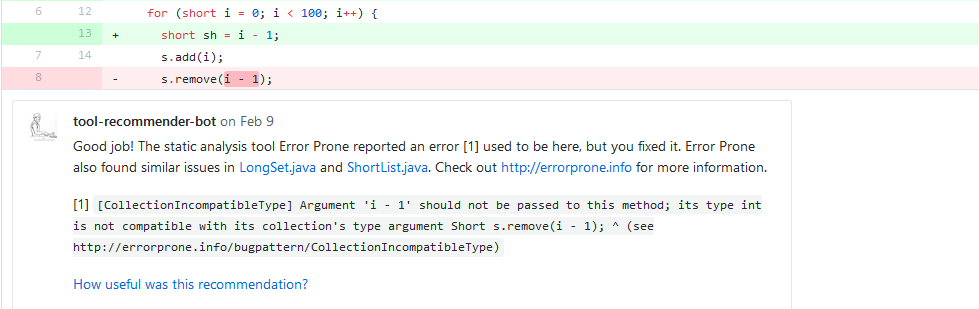
\includegraphics[width=\textwidth]{images/screenshot.png}
	\caption{Screenshot of recommendation from \tool}	
	\label{fig:tool} 
\end{figure*}

\section{Motivation}

Our tool recommendation approach is motivated by previous research in tool discovery and peer interactions.

\subsection{Peer Interactions}

Research suggests recommendations between colleagues is the most effective mode of tool discovery. Murphy-Hill and colleagues interviewed software engineers and found that, even though they appear less frequently in the workplace, developers prefer peer interactions over system-to-user recommendations.~\cite{MurphyHill2011PeerInteraction}~\cite{Murphy-Hill2015HowDoUsers}. Similarly, Welty discovered that software users sought help from colleagues more often than search engines and help menus~\cite{Welty2011Help}. 

To better understand what makes peer interactions effective, Brown and colleagues observed how software users recommend tools to each other while completing tasks. Their results suggest \emph{receptiveness} is a significant factor in determining the outcome of tool recommendations, while other characteristics such as politeness and persuasiveness are not as important~\cite{vlhcc17}. Fogg argues a receptive audience is vital for designing persuasive technology, and describes receptiveness as: 1) demonstrating a desire and 2) familiarity with acquiring a target behavior~\cite{FoggPersuasive}. In this research, our target behavior is the adoption of useful development tools and these two criteria for receptiveness influenced the design principles for our approach for recommending software engineering tools.

\subsubsection{Demonstrate Desire}

Brown and colleages defined demonstrating a desire to adopt a particular behavior as users expressing interest in ``discovering, using, or learning more information'' about a new practice. In software engineering, developers desire to write high-quality programs without errors. This desire is demonstrated by the fact software engineers spend the majority their time testing and debugging programs~\cite{NIST}. Our approach capitalizes on developers' desires to produce mistake-free code by commending developers for their work. To help improve tool adoption among software engineers, our approach analyzes code changes made by developers to determine their intentions, then compliments the developer on their attempt to improve the code quality.

\subsubsection{Familiarity}

Familiarity is also a key part of receptiveness and important in increasing adoption of a target behavior. Fogg suggests users are more likely to adopt a target behavior if they are familiar with it~\cite{FoggPersuasive}. To improve usage of software engineering tools, our approach integrates familiarity. First, we make recommendations based on developers' contributions to recent projects. Scalabrino and colleagues claim code understandability is one of the most important factors for software development, maintenance, debugging, and testing~\cite{Scalabrino2017Understandability}. Developers should be familiar with the project before making changes to the code base. More specifically, our approach apprehends code the developer may also want to change based on their previous update.

\section{Implementation Walkthrough}

To implement our approach, we developed \tool~to recommend the \textsc{Error Prone} static analysis tool to developers on GitHub. This section provides a general overview of how our automated recommendation system works.

\subsection{Commend}

First, a GitHub user makes a change to a repository. \tool~automatically analyzes to commits and pull requests GitHub projects to find opportunities to commend developers when bugs reported by \textsc{Error Prone} are removed. \textsc{Error Prone} is a static analysis tool that uses a suite of defined bug patterns to detect errors in Java code. Static analysis tools like \textsc{Error Prone} are useful for debugging and preventing errors in source code for applications, however they are often underutilized by software engineers~\cite{Johnson2013Why}. More details on how our implementation determines a bug fix can be found in Section 6.2.

\subsection{Apprehend}

Next, \tool~apprehends places where similar opportunities to the code can be made. GitHub should be knowledgeable and familiar with the changes they propose, as well as the code base to which they are contributing. \tool~suggests \textsc{Error Prone} when a reported bug is fixed by a developer in a commit or pull request, but the same error still exists elsewhere in the code. 

\subsection{Recommend}

Finally, \tool~recommends \textsc{Error Prone} to the GitHub user at the location of their fix in the code. We commend developers by telling them ``Good job!'' and presenting the error they fixed. \tool~ provides the apprehended opportunities for similar code changes as links to buggy lines with the same error in other parts of the code. Finally, we provide a link to the \textsc{Error Prone} website for users to learn more about the tool if they are interested. Figure \ref{fig:tool} provides a sample recommendation from \tool~to a developer for \textsc{Error Prone} on a GitHub pull request.

\section{Implementation Description}

This sections provides technical details on the implementation of our approach in \tool. The design of our system is motivated by current practices in the software engineering industry to make \tool~more similar to a peer for developers.

\subsection{Continuous Integration}

To analyze developer changes, our system utilizes continuous integration concepts and tools to observe code modifications to GitHub repositories. \tool~is implemented as a plugin for Jenkins, ``the leading open source automation server'' for source code deployment and delivery.\footnote{https://jenkins.io/} We use Jenkins to periodically check for new modifications, commits and pull requests, to GitHub projects every 15 minutes. Our system ignores any commits or pull requests from developers that do not modify a Java file.
When a new code change is found, Jenkins to automatically analyze the patch and run our approach. 

To analyze the source code, we target projects that use the Maven~\footnote{https://maven.apache.org/} build automation and software dependency management tool for Java applications. We automatically inject \textsc{Error Prone} as a Maven plugin to a repository's project object model file (\textit{pom.xml}) and run the build process with the tool. \tool~builds both the original version of the code before the proposed changes were made (base) and the changed version of the repository with the modifications from the developer (head) to inspect differences. The base and head versions of the source code are tracked using the JGit Java API.\footnote{https://eclipse.org/jgit/}

\subsection{Debugging}

Before commending developers on their work, \tool~must debug to find errors and determine if proposed code changes are a fix. After building the base and head versions with \textsc{Error Prone}, our system parses the output of each build to determine if any faults reported were removed between versions of code. To determine if a change fixes a defect, we developed an algorithm using the code differencing tool GumTree~\cite{GumTree}. GumTree allows us to identify actions (addition, delete, insert, move, and update) performed between the altered versions of the project. 

To determine if an error was fixed, we take several things into consideration: First, we ignore errors that are removed but were not located in a file modified by the developer. This ensures that the GitHub user will be familiar with the code changed and potential error fixed. Second, we ignore changes where only delete actions were detected between the base and head versions of a file. This avoids making recommendations in situations where defects were only removed by developers. For example, deleting a class will remove errors reported by \textsc{Error Prone} in the source code, however the intention was not to fix the bugs. Thus, for a change to be considered a fix there must be new code added or existing code modified by the developer. Similarly, we also ignore classes that are deprecated by developers. These conditions were put in place minimize false positives and prevent errant recommendations to software engineers in our approach.

When a fix is identified in the changed version of code, \tool~finds the location of the fix in the head version. To find the modified line of code that fixed a bug, we use GumTree to parse the source code and convert it to abstract syntax trees. We look for the action closest to the offset of the error node determined from the line number reported by \textsc{Error Prone}. If the closest action is not a delete, then our approach uses the location of that action. Otherwise, our algorithm iteratively searches for the closest sibling node or parent nodes that is not a delete action. To apprehend different opportunities for similar changes, we iterate through the list of errors reported by \textsc{Error Prone} in the head version of code and look for instances of the same error that was fixed by the developer.

\subsection{Code Review}

Code reviews between developers are a standard procedure of software engineering teams to improve code quality~\cite{CodeReviewingTrenches}. This practice also applies to GitHub projects, with many repositories requiring approval from another developer before changes can be merged into the main code base~\cite{PullRequestReview}. Our approach simulates peer code reviews by making recommendations for static analysis tools as a comment on pull requests and commits. Github allows users to make comments on specific lines of code in situ with the code changes. \tool~determines where to automatically make recommendation comments by converting the line number of the identified fix to the equivalent position in the diff file, or textual representation of code changes made in a commit or pull request, represented by the number of lines below the ``@@'' symbol in the header\footnote{https://developer.github.com/v3/pulls/comments/\#create-a-comment}. An example of a comment from \tool~is displayed in Figure \ref{fig:tool}.

To increase the likelihood of tool adoption, \tool~implements our approach by commending developers on their changes, apprehending chances for similar modifications, and recommending software engineering tools to find even more related errors. In the comment, \tool~uses language similar to a peer to compliment the author's code contribution. For instance, our system uses ``Good job!'' to commend developers for fixing an error. Additionally, our system presents similar instances of the fixed error found elsewhere in the code.  \tool~automatically adds direct links to at most two different locations of the same defect where a similar fix can be applied. Finally, we recommend \textsc{Error Prone} and provide information about the tool to encourage developers to use software engineering tools in their future work to fix more related errors and more.

\section{Methodology}

Our study evaluates the effectiveness of \tool~by analyzing how often our system recommends software engineering tools and how developers respond to recommendations from our system.

\subsection{Projects}

We used real-world open source software applications to evaluate \tool. To choose projects for this study from the millions of GitHub repositories online, we used the following criteria:

\begin{itemize}
\item primariy written in Java,
\item build using Maven,
\item do not already use \textsc{Error Prone},
\item ranked among the most popular and most recently updated repositories
\end{itemize}

Our evaluation was limited to Java projects since \textsc{Error Prone} can only analyze Java source code. To determine if a repository used Maven as a build system, we automatically checked if a Project Object Model (\textit{pom.xml}) configuration file was located in the home directory. We also checked to make sure that the pom.xml did not already contain the \textsc{Error Prone} plugin to avoid projects that already use \textsc{Error Prone}. We selected projects that don't use \textsc{Error Prone} to increase awareness of the tool in recommendations. Developers are less likely to know about the tool if the projects they contribute to do not implement it in their build. 

To get the most popular repositories, we filtered GitHub projects by the amount of stars based on numbers in the Fibonnaci sequence. We chose the most starred repositories to study the most popular projects on GitHub. Stars are a social aspect of GitHub where users can indicate their favorite projects and repositories of interest\footnote{https://help.github.com/articles/about-stars/}. Using Fibonacci numbers allowed us to get a higher concentration of projects with a lower amount of stars, while fewer projects will have a very large number of stars. To filter of repositories, we grouped projects with 1 or 2 stars, 2 or 3 stars, between 3 and 5 stars, between 5 and 8 stars, etc., and sorted the top 100 projects in each group by when they were most recently updated. After using a GitHub search API to find projects that met the above criteria, we compiled a list of 789 code repositories. Out of those projects, one repository failed due to broken Unicode text. %TODO: find other failed projects w/ errors
The projects used for our evaluation include a wide range of software applications providing a variety of services from large software companies such as Google and Apache to individual developers. A list of projects used for this study is publicly available online.\footnote{\url{https://gist.github.com/tool-recommender-bot/1769ccd148508beabcd273a731723860}}
%TODO: Maybe examples of projects?

\subsection{Study Design}

To evaluate the effectiveness of our approach, we compared \tool~to different styles and mediums of tool recommendations.

\subsubsection{Setup}

To analyze 700+ GitHub repositories simultaneously, we set up \tool~on virtual machines. We used Ansible\footnote{https://www.ansible.com/} to automatically generate and provision Jenkins jobs for every project. To limit the load on each machine, we ran our study in parallel by dividing the Jenkins jobs among \textit{n} virtual CentOS images. The scripts and instructions to used setup our study environment for \tool~are publicly available to view online.

To test the effectiveness of our approach, we used four different recommendation styles based on our design principles of commending developers for their work and apprehending opportunities to make similar changes. The four recommendation styles include commending and apprehending, commending only, apprehending only, and neither commending nor apprehending. In each case, a recommendation was always made. We adapted \tool~to make recommendations without commending or without apprehending. %TODO: Without commendation,...
Without apprehending, our system simply commends the developer for their fix and does not link to similar errors found in other parts of the code. For the final recommendation without commending or apprehending, we decided to send recommendations to developers by email without commending them for their patch and not providing other instances to make a similar fix. An overview of each style is presented in Table~\ref{table:styles}.


\begin{table*}
\begin{center}
\caption{Study Recommendation Styles}
\begin{tabular*}{\textwidth}{ c|c|p{5cm}|p{5cm}| }
  \multicolumn{2}{ c }{\textbf{}} & \multicolumn{2}{ c }{\textbf{Commend}} \\ \cline{2-4}
 & & Yes & No \\ \cline{2-4}
\multirow{2}{*}{\textbf{Apprehend}} 
	 & Yes & \tool  & Modified \tool~(without commending) \\ \cline{2-4}
	 & No & Modified \tool~(without apprehending) &  Email  \\ \cline{2-4}
\end{tabular*}
\label{table:styles}
\end{center}
\end{table*}


\subsubsection{Recommendation Review}

Johnson and colleagues discovered one of the primary barriers to static analysis tool usage among software engineers is false positives in the output~\cite{Johnson2013Why}. To prevent unnecessary recommendations from our system, we manually reviewed all instances where \tool~reported a recommendation should be made. After inspecting each repository modification, \tool~determines whether it is an appropriate case to make a recommendation to the developer. For this study, we streamlined this process to send an email for the authors to review if a recommendation was proposed by our system. After the authors reviewed the code changes, if we deemed it was a true positive case we proceeded to use \tool~to post the comment recommending \textsc{Error Prone} to the developer on the pull request or commit. Otherwise, we noted the instance of a false positive in our approach and did not make the recommendation. In situations where one repository code change provided multiple opportunities for a recommendation, the authors examined each of the changes and selected one of the errors reported as fixed to recommend to the developer.

\subsubsection{Debriefing}

To gather data on the usefulness of our system, we sent a follow-up survey to developers. Survey participants were users who received a recommendation from \tool~on their pull request or commit. We asked developers about their awareness of \textsc{Error Prone} and how likely they are to use the tool in the future. The survey also included a free-response section to provide an opportunity for participants to add comments on the usefulness of the recommendation.

Developers voluntarily consented to complete the survey and provide feedback on our system. To ensure developers answered honestly, we notified respondents that their answers will be used for research purposes. Previous research has shown that survey participants are more motivated to answer truthfullly if they know they are contributing to research~\cite{Krosnick1991Research}. 

To futher examine the effectiveness of \tool, we compared our approach to sending email recommendations to developers. To study this, we found similar instances of code fixes by GitHub users where our system would recommend a tool and, instead of making the recommendation with \tool~on the pull request or commit, send an email suggesting \textsc{Error Prone} to the developers. The emails also contained the recommendation feedback survey for developers, and we compared results to see how software engineers responded to receiving a recommendation by email vs. on GitHub from \tool. To send a recommendation via email, the developer must have an email address publicly available on the GitHub user profile. 

\subsection{Data Analysis}

We analyzed the data collected in our study to determine effectiveness of our automated tool recommendation system.

\subsubsection{Quantitative}

To determine the effectiveness of our approach, we observed how often\tool~makes recommendations on commits and pull requests. In addition to the frequency of recommendations, we also tracked instances where \textsc{Error Prone} defects were removed but not reported as fixed according to our fix identification algorithm in Section III.B.2, the number of occurrences where errors were fixed but no other instances of that bug were found in the code, and the false positive rate.

Effective tool recommendation systems should have ample opportunities to regularly make recommendations to users. To determine how often \tool~automatically recommends \textsc{Error Prone}, we observed the total number of new pull requests and commits, and compared it to the amount recommendations made by our tool. We calculated the rate of true positive recommendations during the span of our study to measure the recommendation rate for each GitHub repository used in our evaluation. To calculate the false positive rate, we compared the number of unnecessary instances where our tool proposed a recommendation found by the authors to the total number of instances where a recommendation reported by \tool.

\subsubsection{Qualitative}

For our second research question, we accumulated responses from developers in our follow-up survey presented in recommendations from \tool~and by email to determine the usefulness of our system. We utilized a five-point Likert scale for participants to rank how knowledgeable they were about the existence of \textsc{Error Prone} before the recommendation and how likely they are to use \textsc{Error Prone} for future development tasks. An optional free response section was provided at the end for respondents to describe explain why or why not they found the recommendation useful. These responses were used to analyze developers' reactions to our automated recommendation. Finally, researchers analyzed and independently coded open-ended responses from participants to further analyze the effectiveness of our approach based on feedback from software developers. We measured the response rate by observing the total number of recommendations made, the total number of survey responses, and the positive and negative responses from developers who received a recommendation via \tool~and via email.

\section{Results}

\subsection{Quantitative}

Tons of recommendations... \\

No false positives...

\subsection{Qualitative}

\subsubsection{Recommend}

\subsubsection{Commend, Recommend}

\subsubsection{Apprehend, Recommend}

\subsubsection{Commend, Apprehend, Recommend}

Excellent responses from recommendees...\\

Something statistically significant...

\section{Discussion}

\subsection{Observations}

\subsubsection{Why Were There So Few Recommendations?}

Non-java changes, number of errors removed but not fixed, number of errors fixed without another instance in the code, manual inspection of pull requests and commits...

\subsection{Implications}

Here's what our results say about improving tool recommendation systems...

\section{Limitations}

An internal threat to the validity of this work is our use of code differencing to determine if developers intended to fix a bug in a commit or pull request. We cannot definitively determine the intentions of GitHub developers making changes to a repository, however two authors analyzed the code changes and came to an agreement on if the modified patch was a fix before making a recommendation to the developer. Additionally, although we used a Likert scale to measure if GitHub users who received a recommendation were likely to use \textsc{Error Prone} in the future, we did not measure if the tool was actually adopted by the developers for future tasks.

Our evaluation has limited generalizablility due to the fact we only assessed recommendations for the \textsc{Error Prone} static analysis tool. This restricted our study to evaluate Java projects and a specific set of errors that can be reported by the tool. We selected \textsc{Error Prone} because it is able to report a wide variety of errors based on bug patterns for Java code. Another external threat to the validity of this study is the projects selected for our evaluation. We only examined open source repositories on GitHub, and these results may not generalize to developers of closed source software or projects on other code hosting sites, such as BitBucket.\footnote{http://bitbucket.org} To minimize this threat, we evaluated \tool~on a large number of popular software applications on GitHub that provide many different services from a wide variety of software companies and developers. 

\section{Future Work}

The main goal of our future work is to increase the practicality of \tool~for researchers and toolsmiths to implement our approach with their tools. A next step is to implement our approach with multiple static analysis tools, such as Checkstyle\footnote{http://checkstyle.sourceforge.net/} for Java. This will allow us to have more opportunities to make recommendations to developers based on the output from different tools. Additionally, we plan to update our system to work with software engineering tools that integrate as plugins for different build systems such as Gradle\footnote{https://gradle.org/} and Travis CI\footnote{https://travis-ci.org/}, as opposed to just Maven projects. Future work will also extend \tool~to work with different types of tools to increase adoption and usage, for example Find Security Bugs\footnote{https://find-sec-bugs.github.io/} which is useful for finding security vulnerabilities in Java web applications. Finally, future work will consist of expanding \tool~to work with software engineering tools for different programming languages, such as the Pylint\footnote{https://www.pylint.org/} static analysis tool for Python, clang\footnote{https://clang.llvm.org/} compiler and static analyzer for C and C++, and more.



\section{Conclusion}

\tool~is awesome

%\balance
%\section{Acknowledgments}

%Thanks to all of the student and professional data analysts who volunteered for this study.

% The following two commands are all you need in the
% initial runs of your .tex file to
% produce the bibliography for the citations in your paper.
\bibliographystyle{abbrv}
\bibliography{paper}  
% You must have a proper ''.bib'' file
%  and remember to run:
% latex bibtex latex latex
% to resolve all references
%
% ACM needs 'a single self-contained file'!

%% That's all folks!
\end{document}
